\documentclass[../main.tex]{subfiles}
\begin{document}
  \chapter{Basic definitions}


    \section{Organization}
    Course web page: \url{https://www.fuw.edu.pl/~mklis/hydro2022.html}
    

    Requirements to obtain credit:
    \begin{itemize}
      \item Homework ($30\%$),
      \item Midterm exam ($35\%$),
      \item Written exam ($35\%$),
      \item Oral exam (optional, only improves).
    \end{itemize}

    % Climate is a nice playground for hydrodynamics.

    \section{Basic laws}

    \begin{example}
      Out of context Navier-Stokes equations:
      \begin{displaymath}
        \ptf{\vec u}{t} + \vec u \cdot \nabla \vec u = - \frac{1}{\rho} \nabla p + \nu\nabla^2 \vec u,
      \end{displaymath}
      \begin{displaymath}
        \nabla \cdot \vec u = 0.
      \end{displaymath}
      where $\vec u(\vec r,t)$ is a fluid velocity vector field, $\rho(\vec r,t)$ is a fluid density, 
      $p(\vec r, t)$ is a pressure, $\nu$ is a kinematic viscosity.
    \end{example}

    \sep


    Continuum hypothesis states that
    \begin{displaymath}
      \rho = \frac{\delta\eta}{\delta \nu},
    \end{displaymath}
    where $\eta$ is a number of particles in a region and $\nu$ is a volume of this region.
    Of course if the volume $\nu$ is small enough $\rho$ is may vary a lot (obviously it may not even be continuous).
    There is however such volume $V$ which is ,,big enough'', so that for $\nu > V$ $\rho$ does not vary ,,that much''.

    \begin{figure}[h]
      \begin{center}
        \begin{subfigure}{0.3\linewidth}
          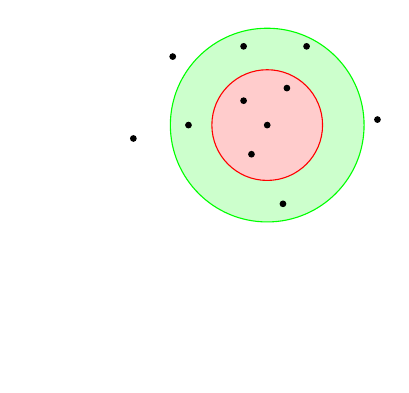
\begin{tikzpicture}
            \draw[white] (0,0) circle (1pt);
            \begin{scope}[shift={(3cm, 3cm)}]
              \draw[fill=green!20, draw=green] (0,0) circle (35pt);
              \filldraw[fill=red!20, draw=red] (0,0) circle (20pt);
              \filldraw[black] (0,0) circle (1pt);
              \filldraw[black] (0.5,1) circle (1pt);
              \filldraw[black] (-0.3,1) circle (1pt);
              \filldraw[black] (0.2,-1) circle (1pt);
              \filldraw[black] (-1,0) circle (1pt);
              \filldraw[black] (-0.3,0.31) circle (1pt);
              \filldraw[black] (0.25,0.47) circle (1pt);
              \filldraw[black] (-0.20,-0.37) circle (1pt);
              \filldraw[black] (-1.7,-0.17) circle (1pt);
              \filldraw[black] (-1.2,0.87) circle (1pt);
              \filldraw[black] (1.4,0.07) circle (1pt);
            \end{scope}
          \end{tikzpicture}
        \end{subfigure}%
        \begin{subfigure}{0.7\linewidth}
          \centering
          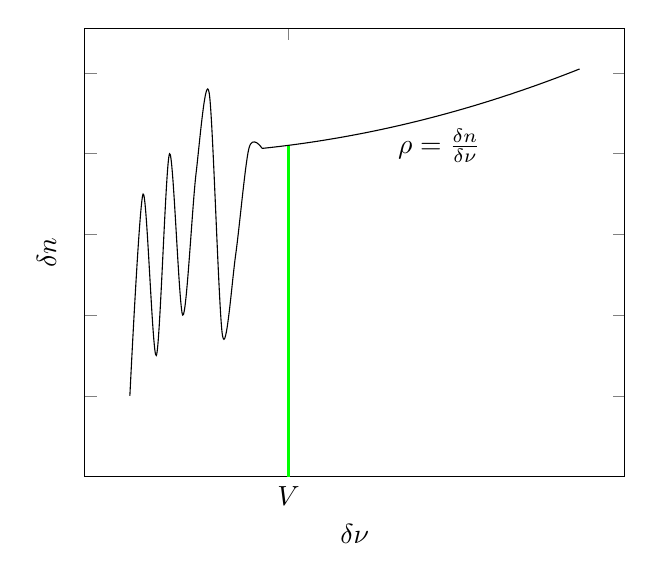
\begin{tikzpicture}
            \begin{axis}[
                xtick = {13},
                xticklabels = {$V$},
                yticklabels = {},
                ymin=0,
                xlabel = {$\delta \nu$},
                ylabel = {$\delta n$}
              ]
              \addplot[smooth] coordinates {
                (1, 2)
                (2, 7)
                (3, 3)
                (4, 8)
                (5, 4)
                (6, 7.5)
                (7, 9.5)
                (8, 3.5)
                (9, 5.5)
                (10, 8.132)
                (11, 8.132)
                % (12.5, 8.1)
                % (15, 8.3)
                % (17.5, 8.5)
                % (20, 9)
                % (30, 9.5)
              };
              \addplot [
                domain = 11:35,
                samples = 100
              ]
              {0.01 * (0.2 * x^2 - x + 800)};
              \addplot +[mark=none, color=green, thick] coordinates {(13, -1) (13, 8.2)};

            \end{axis}
              \node at (4.5, 4.2) {$\rho = \frac{\delta n}{\delta \nu}$};
          \end{tikzpicture}
        \end{subfigure}

      \end{center}
      \label{fig:0}
    \end{figure}


    Since matter is not continuous, we can't speak of a density at a point (in a mathematical sense) and
    thus, when we use the phrase ,,point'' we mean ,,at a point for homogeneous physical system''.

    We also introduce length scale separation % for 

    \begin{displaymath}
      \begin{matrix}
        \tm{molecular length scale} & \ll & \nu^{\frac{1}{3}} & \ll & L.
      \end{matrix}
    \end{displaymath}
    We call those characteristic length scales ,,\emph{micro}'', ,,\emph{muso}'' and ,,\emph{macro}'' respectively.
    

    \subsection{Equilibrium thermodynamics}
    \begin{figure}[H]
      \begin{subfigure}{0.5\linewidth}
        \centering
        \begin{tikzpicture}
          \node[anchor = south west] (image) at (0,0)
          {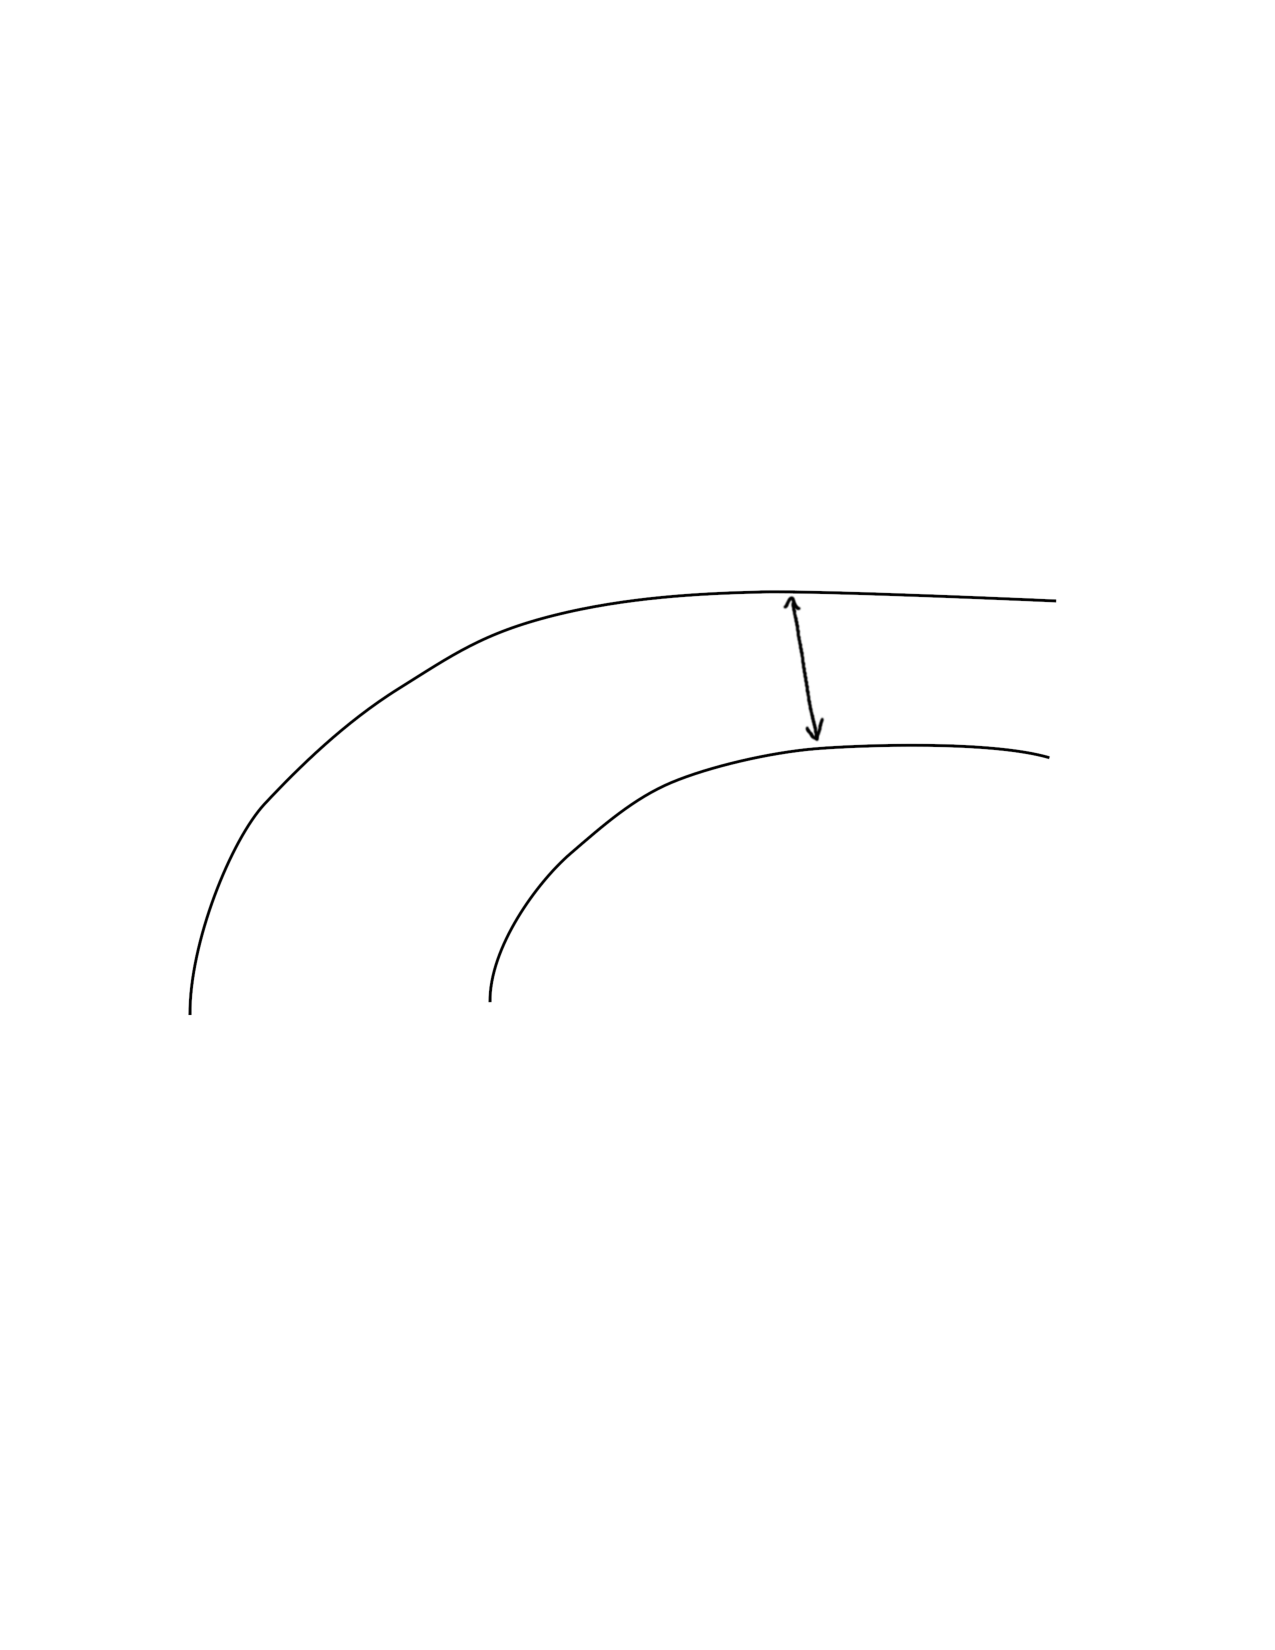
\includegraphics[width=\textwidth]{../images/00river.pdf}};
          \begin{scope}[x={(image.south east)}, y={(image.north west)}]
            \node at (0.35, 0.5) {$\vec u(\vec r, t)$};
            \node at (0.65, 0.5) {river};
            \draw [-stealth] (0.4,0.52) -- (0.5,.58);
          \end{scope}
        \end{tikzpicture}

      \end{subfigure}
      \begin{subfigure}{0.5\linewidth}
        \centering
        \begin{tikzpicture}
          \node[anchor=south west] (image) at (0,0)
          {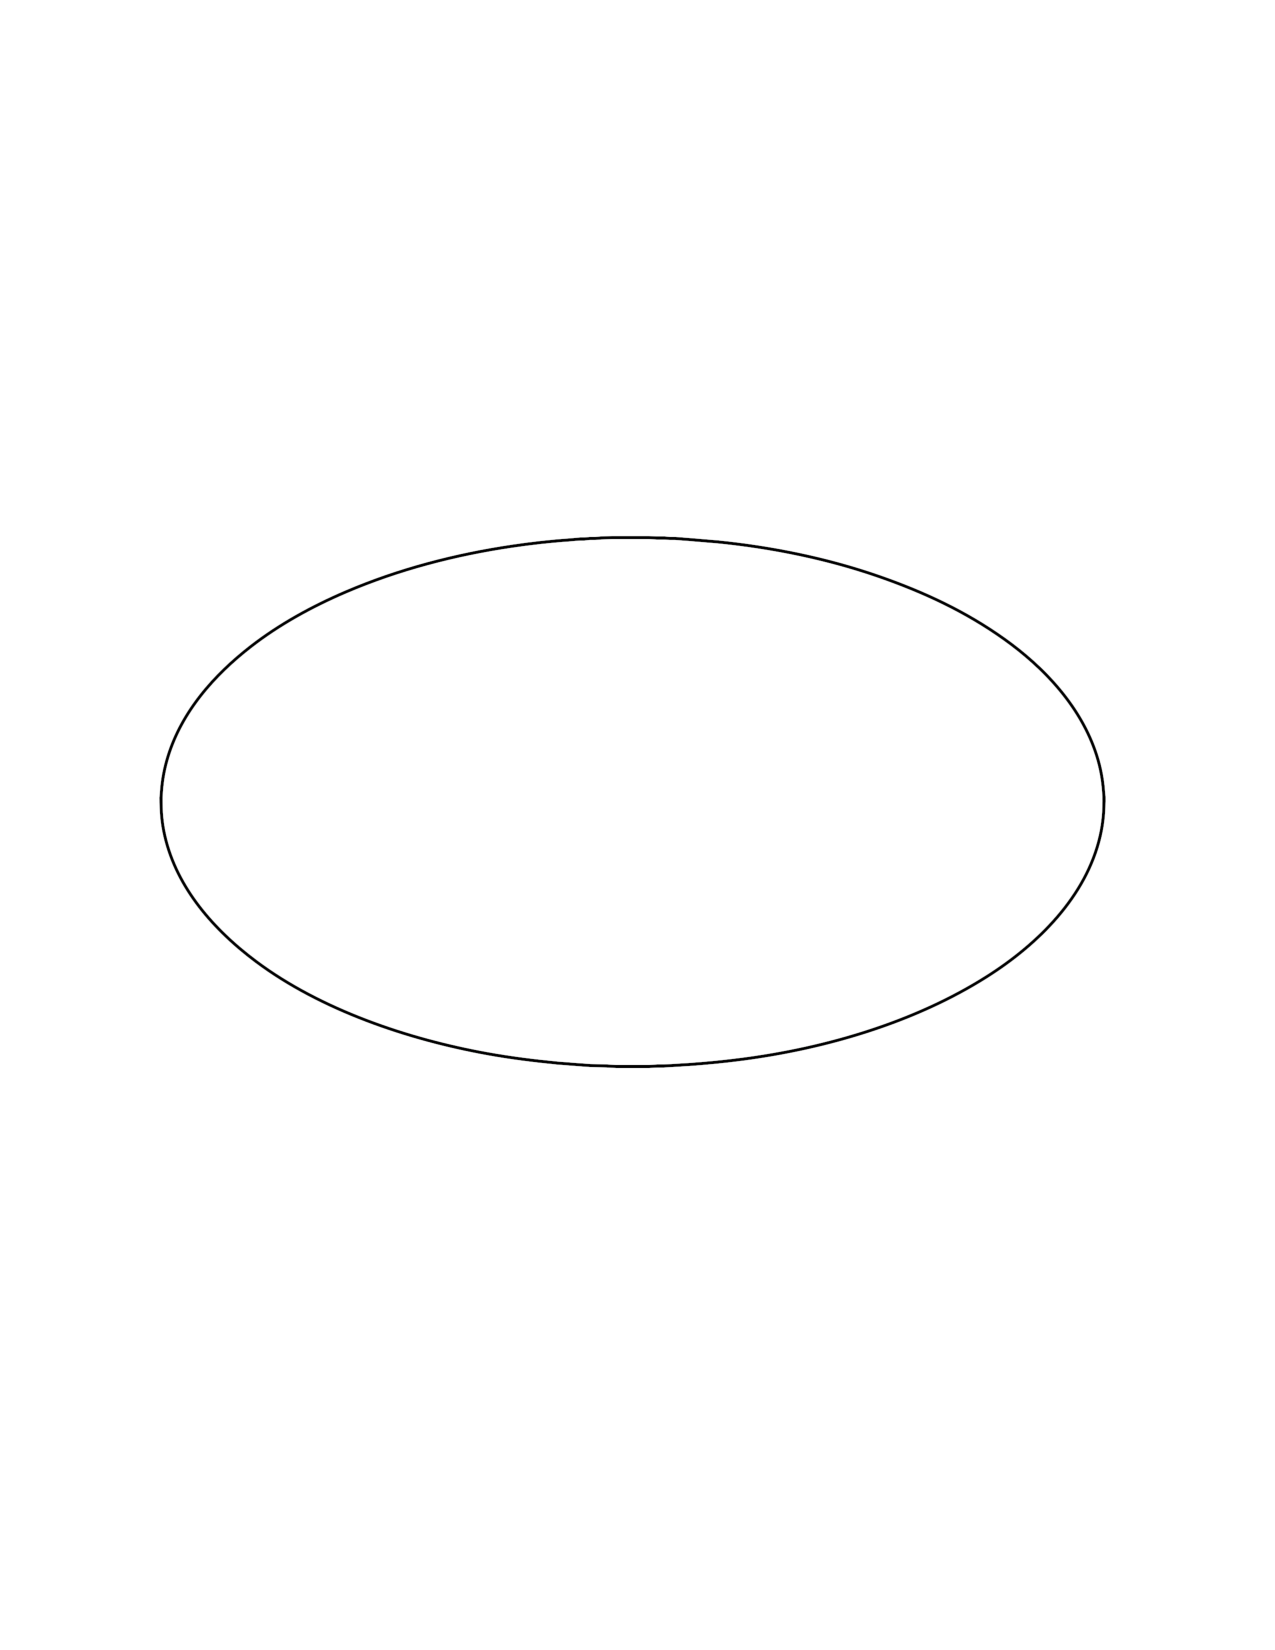
\includegraphics[width=\textwidth]{./images/00ellipse.pdf}};
          \begin{scope}[x={(image.south east)}, y={(image.north west)}]
            \node at (0.3, 0.5) {$N, m$};
            \node at (0.43, 0.58) {$\vec u$};
            \draw [-stealth] (0.4,0.52) -- (0.5,.58);
          \end{scope}
        \end{tikzpicture}
      \end{subfigure}
    \end{figure}


    Let us examine an example of a water in a river.
    Assume that the water has some velocity $\vec {u}$, momentum $\vec{P}$ and also that it can 
    exchange mass and heat, the latter given by $\d Q = T \d S$.
    Therefore an incremental change in the energy of this system can be expressed as
    \begin{displaymath}
      \d E = \vec u \cdot \d \vec P - p \d V + T \d S + \mu \d N,
    \end{displaymath}
    where $\mu$ is the chemical potential of the system.
    Thus
    \begin{displaymath}
      E = E(\vec P, V, S, N).
    \end{displaymath}
    This is the \fndef{energy representation} of a thermodynamical system.
    Comparing the equations above we obtain
    \begin{displaymath}
      \d E = \underbrace{\ptf{E}{\vec P}}_{\vec u} \d \vec P + \underbrace{\ptf{E}{V}}_{- p} \d V 
      + \underbrace{\ptf{E}{S}}_{T} \d S + \underbrace{\ptf{E}{N}}_{\mu} \d N,
    \end{displaymath} % TODO add some explanation about the fact that \ptf{E}{\vec P} = \vec u.
    Those are called the Gibbs relation for $E$.

    If we want to compute it for a fixed entropy we get
    \begin{displaymath}
      \d S = \frac{1}{T} \d E - \frac{\vec u}{T} \d \vec P + \frac{p}{T} \d V - \frac{\mu}{T} \d N.
    \end{displaymath}
    Thus
    \begin{displaymath}
      S = S(E, \vec P, V, N), \quad
      \d S = \underbrace{\ptf{S}{E}}_{\frac{1}{T}} \d E + \underbrace{\ptf{S}{\vec P}}_{- \frac{\vec u}{T}} \d \vec P 
      + \underbrace{\ptf{S}{V}}_{\frac{p}{T}} \d V + \underbrace{\ptf{S}{N}}_{- \frac{\mu}{T}} \d N,
    \end{displaymath}
    Those are Gibbs relations for $S$.

    It is very tricky to control entropy --- it's much easier to control the temperature.
    To obtain a description of our system when $T$ is an independent variable we need to use another thermodynamical potential,
    % switch variables i.e. use other thermodynamical potential.
    which is Helmholz free energy.
    Transition is obtained by
    \begin{displaymath}
      (S \ra T) \quad F = E - TS, \quad F = F(\vec P, V, T, N)
    \end{displaymath}
    \begin{displaymath}
      \d F = - S \d T - p \d V  + \vec{u} \d \vec {P}  + \mu \d N.
    \end{displaymath}
    Now we can do the same to switch other variables. Thus we obtain
    \begin{displaymath}
      (V \ra P) \quad H = E + p V, \quad H = H(\vec P, p, S, N),
    \end{displaymath}
    which is called an enthalpy,
    \begin{displaymath}
      (S \ra T) \quad G = E + pV - TS, \quad G = G(\vec P, p , T, N),
    \end{displaymath}
    which is called a Gibbs potential.

    Now we want to consider if they are Galilean invariant
    % \todo Fig\#4.

    % \begin{figure}[ht]
    %   \centering
    %   \begin{tikzpicture}
    %     \node[anchor=south west] (image) at (0,0)
    %     {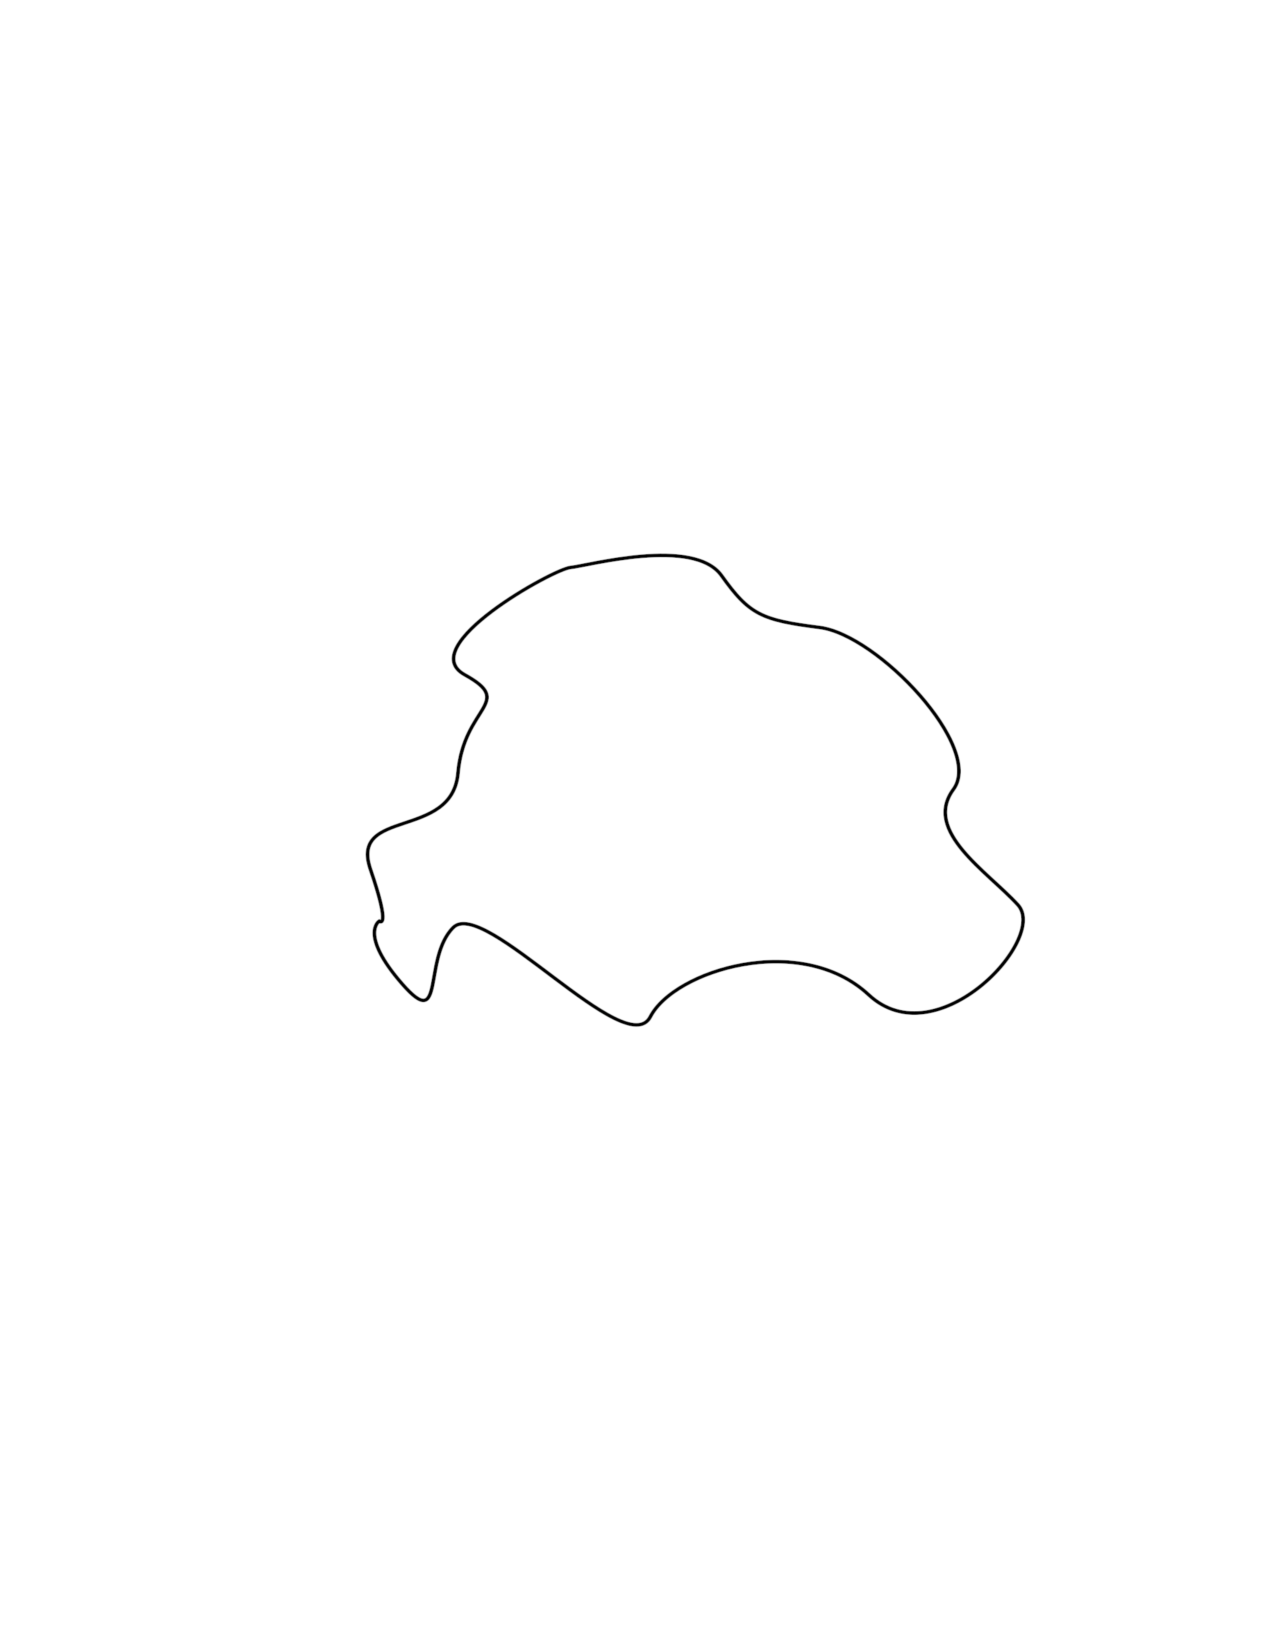
\includegraphics[width=0.5\textwidth]{./images/00splash.pdf}};
    %     \begin{scope}[x={(image.south east)}, y={(image.north west)}]
    %       \node at (0.3, 0.5) {$N, m$};
    %       \node at (0.43, 0.58) {$\vec u$};
    %       \draw [-stealth] (0.4,0.52) -- (0.5,.58);
    %     \end{scope}
    %   \end{tikzpicture}
    % \end{figure}

    \begin{displaymath}
      E(\vec P, V, S, N) = E_0 (V, S, N) + \frac{\vec P^2}{2 M},
    \end{displaymath}
    where $E_0$ is the \fndef{internal energy}.
    For other potentials we obtain
    \begin{displaymath}
      H(\vec P, p , S, N) = H_0(p, S, N) + \frac{\vec P^2}{2 M},
    \end{displaymath}
    \begin{displaymath}
      F(\vec P, V, T, N) = F_0(T, V, N) + \frac{\vec P^2}{2 M},
    \end{displaymath}
    \begin{displaymath}
      G(\vec P, V, T, N) = G_0(T, p, N) + \frac{\vec P^2}{2 M}.
    \end{displaymath}
    
    Using $\vec P = M \vec u$ we get
    \begin{displaymath}
      E = E_0 + \frac{1}{2} M \vec u ^2.
    \end{displaymath}
    \begin{displaymath}
      \d E = \d E_0 + \vec u \cdot \d \vec P,
    \end{displaymath}
    \begin{displaymath}
      \d S = - \frac{1}{T} \vec u \cdot \d \vec P + \frac{1}{T} \d E + \frac{p}{T} \d V - \frac{\mu}{T} \d N,
    \end{displaymath}
    \begin{displaymath}
      \d S = \frac{1}{T}\d E_0 + \frac{p}{T} \d V - \frac{\mu}{T} \d N 
      \qLRa S(\vec P , E , V, N) = S(E_0, V, N).
    \end{displaymath}
    Thus $S$ is a Galilean invariant.

    \subsection{Heterogenous macroscopic system}
    % \todo Fig\#5

    \begin{figure}
      \centering
       \begin{tikzpicture}
         \node[anchor=south west] (image) at (0,0)
         {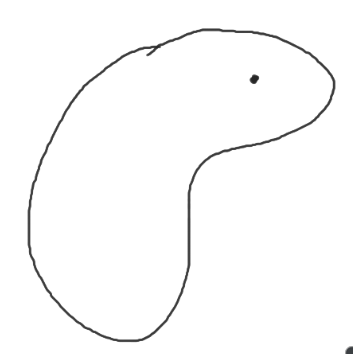
\includegraphics[width=0.25\textwidth]{./images/00Fig5.png}};
         \begin{scope}[x={(image.south east)}, y={(image.north west)}]
           \node at (0.6, 0.7) {$v = \d\vec r$}; % TODO what does it mean XD
           \node at (0.35, 0.15) {$\Omega$}; % TODO what does it mean XD
           \node at (0.95, 0.45) {$\mathbb{M} = \int_\Omega \rho(\vec r, t) \d \vec r$}; % TODO what does it mean XD
           \node at (0.95, 0.25) {$\mathbb{E} = \int_\Omega \epsilon(\vec r, t) \d \vec r$}; % TODO what does it mean XD
         \end{scope}
       \end{tikzpicture}
      \caption{Sample volume $\Omega$. $\rho$ stands for mass density, $\varepsilon$ for density of the system.}
      \label{fig:1.5}
    \end{figure}

    ,,Densities'' are extensive properties per unit volume.
    Assume that $V = \const$, $\d V = 0$.
    Example of densities
    \begin{itemize}
      \item $\rho = \frac{M}{V}$ mass density,
      \item $\vec j = \frac{\vec P}{V}$ momentum density,
      \item $\varepsilon = \frac{E}{V}$ energy density,
      \item $\sigma = \frac{S}{V}$ entropy density.
    \end{itemize}
    \begin{displaymath}
      \d E = \vec u \d \vec P - p \d V + T \d S + \mu \d N / \cdot \frac{1}{V}.
    \end{displaymath}
    \begin{displaymath}
      \d \varepsilon = \vec u \cdot \d \vec j + T \d \sigma + \mu\d n, \quad \d n = \frac{\d \rho}{m},
    \end{displaymath}
    \begin{displaymath}
      \rho = \frac{M}{V} = \frac{Nm}{V} = nm \qLRa \d n = \frac{\d \rho}{m}.
    \end{displaymath}
    Thus the energy fundamental representation in terms of densities can be written as
    \begin{displaymath}
      \varepsilon = \varepsilon(\vec j, \sigma, \rho).
    \end{displaymath}
    After performing a Galilean transform we get
    \begin{displaymath}
      \varepsilon(\vec j, \sigma, \rho) = \varepsilon_0(\sigma, \rho) + \frac{1}{2} \rho \vec u ^2.
    \end{displaymath}
    
    We can do the same to represent entropy in terms of densities
    \begin{displaymath}
      \d S = \dots \frac{1}{V} \qLRa  \d \sigma = \frac{1}{T} \d \varepsilon_0 - \frac{1}{T} \frac{\mu}{m} \d p.
    \end{displaymath}
    Thus
    \begin{displaymath}
      \sigma = \sigma(\varepsilon_0, \rho),
    \end{displaymath}
    which is also Galilean invariant.


    \subsection{Flow of Heterogenous macroscopic system}
    We are using thermodynamics equilibrium despite the fact that the system flows (which means that it is \emph{not} in the equilibrium).
    However there is no contradiction if we assume local, thermodynamical equilibrium.
    The same assumption is made in Navier-Stokes equations.

    From now one we use pseudostatic transition.
    The difference between quasi-static and pseudostatic is that pseudostatic need not to be reversible.
    Forces which acts during quasi-static transformation are those which keeps the system in equilibrium.
    Example of pseudostatic transition which is not quasi-static is a flow of viscose fluid.
    % \todo Fig\#6.

    \begin{figure}
      \centering
       \begin{tikzpicture}
         \node[anchor=south west] (image) at (0,0)
         {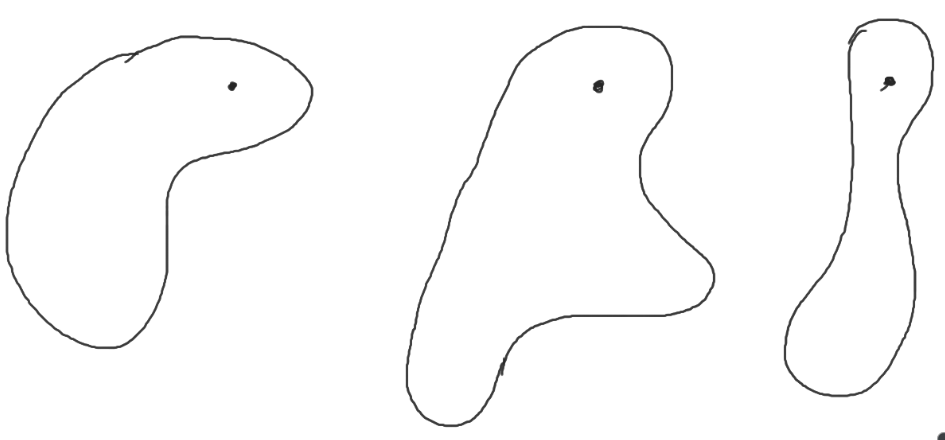
\includegraphics[width=0.45\textwidth]{./images/00Fig6.png}};
         \begin{scope}[x={(image.south east)}, y={(image.north west)}]
           \node at (0.4, 0.9) {$\varepsilon(\vec j, \sigma, p)$}; 
           \node at (0.4, 0.75) {$\sigma(\varepsilon_0, p)$}; 
           \node at (0.2, 0.15) {$\Omega(t_1)$}; 
           \node at (0.6, 0.15) {$\Omega(t_2)$}; 
           \node at (0.9, 0.15) {$\Omega(t_3)$}; 
         \end{scope}
       \end{tikzpicture}
      \label{fig:1.6}
    \end{figure}
    
    
    \subsection{Kinematics}

    We have two descriptions: Eulerian and Lagrangian.
    Transition between them is obtained by
    % (\todo Fig\#7) 

    \begin{figure}
      \centering
       \begin{tikzpicture}
         \node[anchor=south west] (image) at (0,0)
         {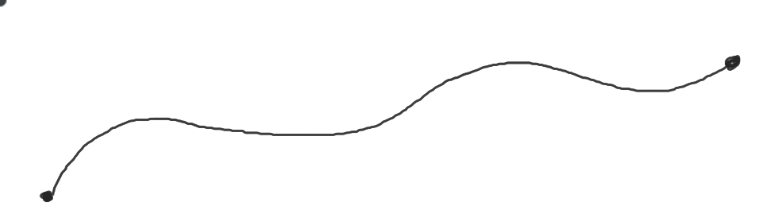
\includegraphics[width=0.25\textwidth]{./images/00Fig7.png}};
         \begin{scope}[x={(image.south east)}, y={(image.north west)}]
           \node at (0.2, 0.1) {$\vec R$}; 
           \node at (0.9, 0.9) {$\vec r(\vec R, t)$}; 
         \end{scope}
       \end{tikzpicture}
      \label{fig:1.7}
    \end{figure}

    

    the solutions to the initial problem
    \begin{displaymath}
      \dfrac{\vec r}{t} = \vec u(r,t), \quad \vec r(t = 0) = \vec R.
    \end{displaymath}

    We want to find dependence of densities as the particle move, and those are
    \begin{center}
      \begin{tabular}{c|c|c|}
        & Euler & Lagrange \\
        \hline
        velocity & $\vec u(r, t) $ & $\vec u[ r(t), t]$\\
        density & $\rho(r, t)$ & $\vec \rho[ r(t), t]$\\
        \hline
      \end{tabular}
    \end{center}
    \begin{displaymath}
      \dfrac{\vec u}{t} = ?, \quad \dfrac{\rho}{t} = ?.
    \end{displaymath}
    
    To do that define $\beta = (\vec u, \rho, S, \sigma, \dots)$. 
    We want to find how $\beta$ change while following the motion 
    of the particle $r(t)$.
    \begin{displaymath}
      \dfrac{\beta}{t} = \dfrac{\beta[\vec r(t),t]}{t} = \ptf{\beta}{t} + \dfrac{r_1 }{t} \ptf{\beta}{r_1} 
      + \dfrac{r_2}{t} \ptf{\beta}{r_2} 
      + \dfrac{r_3}{t} \ptf{\beta}{r_3}  
    \end{displaymath}
    \begin{displaymath}
      = \ptf{\beta}{t} + \vec u (t)\cdot \nabla \beta 
      = \ptf{\beta}{t} + \d \beta(\vec u(t)).
    \end{displaymath}

    \begin{figure}
      \centering
       \begin{tikzpicture}
         \node[anchor=south west] (image) at (0,0)
         {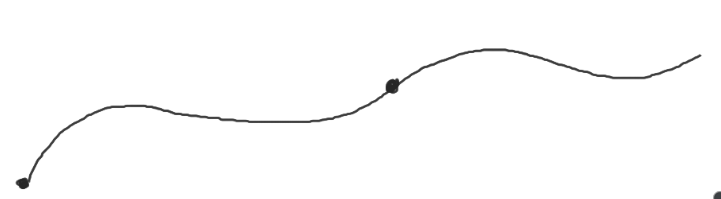
\includegraphics[width=0.25\textwidth]{./images/00Fig8.png}};
         \begin{scope}[x={(image.south east)}, y={(image.north west)}]
           \node at (0.2, 0.1) {$\vec R$}; 
           \node at (0.7, 0.4) {$\beta(\vec r(t), t)$}; 
         \end{scope}
       \end{tikzpicture}
      \label{fig:1.8}
    \end{figure}


    Equation 
    \begin{equation}
      \dfrac{\beta}{t} = \ptf{\beta}{t} + \vec u(t) \cdot \nabla \beta,
      \label{eq:1}
    \end{equation}
    shows a relationship between Eulerian and Lagrangian world, because
    $\dfrac{\beta}{t}$ is a typical Lagrangian while fields (like $\vec u(t)$) are common in Euler's description.
    (Fields are Eulerian objects).
    We introduce a \fndef{total (material) derivative} as 
    \begin{displaymath}
      \dfrac{\dots}{t} = \underbrace{\ptf{\dots}{t}}_{\tm{local derivative}} + \underbrace{\vec u \cdot \nabla(\dots)}_{\tm{advective derivative}}.
    \end{displaymath}
    
    Acceleration of fluid particle
    \begin{displaymath}
      \beta = \vec u \qLRa \dfrac{\beta}{t} = \dfrac{\vec u}{t}.
    \end{displaymath}
    Consider converging chanell with a stationary flow, i.e. $\ptf{\vec u}{t} = 0$.

    % Fig\#9.

    \begin{figure}
      \centering
      \begin{tikzpicture}
        \node[anchor=south west] (image) at (0,0)
        {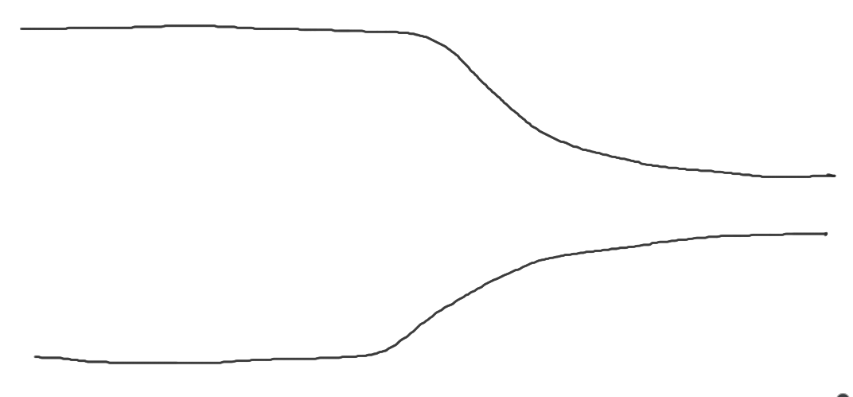
\includegraphics[width=0.25\textwidth]{images/00Fig9.png}};
          \begin{scope}[x={(image.south east)}, y={(image.north west)}]
          \node at (0.1, 0.6) {$\vec v_1$};
          \draw [-stealth] (0.1, 0.5) -- (0.2, 0.5);
          \node at (0.1, 0.3) {$r_1$};

          \node at (0.7, 0.6) {$\vec v_2$};
          \draw [-stealth] (0.7, 0.5) -- (0.9, 0.5);
          \node at (0.7, 0.3) {$r_2$};
          \end{scope}
      \end{tikzpicture}
      \label{fig:1.9}
    \end{figure}

    

    With that in mind
    \begin{displaymath}
      \dfrac{\vec u}{t} = \ptf{\vec u}{t} + \vec u \cdot \nabla \vec u = \vec u \cdot \nabla \vec u.
    \end{displaymath}
    The term $\vec u \cdot \nabla \vec u$ should be interpreted as follows.
    Treat $\vec u$ as a map $\vec u(\vec r): \RR^3 \ra \RR^3$. 
    Thus $\nabla \vec u$ is just a map $D \vec u: \RR^3 \ra \RR^3$ expressed by a matrix
    \begin{displaymath}
      \vec u(\vec r) = \begin{bmatrix}
        u_1 (r_1, r_2, r_3)\\
        u_2 (r_1, r_2, r_3)\\
        u_3 (r_1, r_2, r_3)
      \end{bmatrix}, \quad 
      D \vec u = \begin{bmatrix}
        \ptf{u_1}{r_1} & \ptf{u_1}{r_2} & \ptf{u_1}{r_3} \\
        \ptf{u_2}{r_1} & \ptf{u_2}{r_2} & \ptf{u_2}{r_3} \\
        \ptf{u_3}{r_1} & \ptf{u_3}{r_2} & \ptf{u_3}{r_3}
      \end{bmatrix}.
    \end{displaymath}
    Therefore inner product $\vec u \cdot \nabla \vec u$ really means
    \begin{displaymath}
      \vec u \cdot \nabla \vec u = (D \vec u)(\vec u).
    \end{displaymath}
    At least I think so\dots
    

    
    The term $\vec u \cdot \nabla \vec u$ is called a \fndef{convective acceleration}.
    Although the flow is stationary, the particle experiences acceleration related to movement along the flow lines. 
    
    
    We can interpret the fluid flow as a mapping which takes one point and maps it to the other.

    % Fig\#10.
    \begin{figure}
      \centering
      \begin{tikzpicture}
        \node[anchor=south west] (image) at (0,0)
        {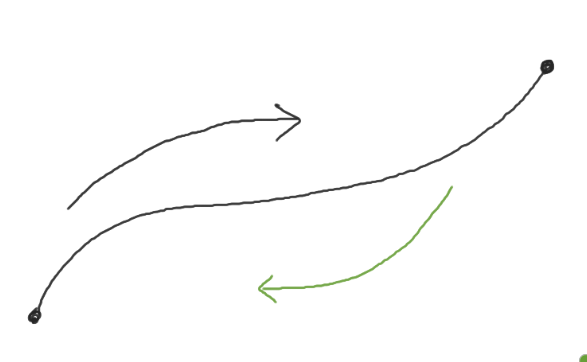
\includegraphics[width=0.35\textwidth]{images/00Fig10.png}};
          \begin{scope}[x={(image.south east)}, y={(image.north west)}]
            \node at (0.3, 0.8) {$r(\cdot)$};
            \node at (0.6, 0.1) {$r^{-1}(\cdot)$};
          \end{scope}
      \end{tikzpicture}
      \label{fig:1.10}
    \end{figure}

    
    
    \paragraph{Streakline}

    \begin{figure}
      \centering
      \begin{tikzpicture}
        \node[anchor=south west] (image) at (0,0)
        {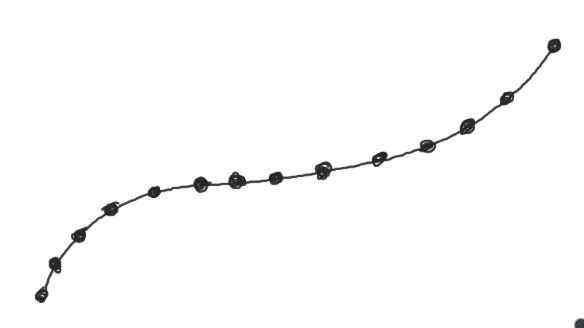
\includegraphics[width=0.25\textwidth]{images/00Fig11.png}};
          \begin{scope}[x={(image.south east)}, y={(image.north west)}]
            \node at (0.0, 0.2) {$\vec y$};
            \node at (0.8, 0.9) {$\vec r(\vec y, t)$};
          \end{scope}
      \end{tikzpicture}
      \caption{Streakline is a line made of all particles that for time $s$, $0 \leq s \leq t$ 
      passed through a fixed point $\vec y$.}
      \label{fig:1.11}
    \end{figure}

    

    Imagine a cigarette and assume that there is no diffusion. 
    The smoke is made out of small, fluid particles.
    The flow line is made out of fluid particles which were passing through $\vec y$ in the time interval
    $0 \leq s \leq t$.
    Suppose that we froze time at $t = t_0$.
    Choose point $A$.
    \fndef{Streakline} through the point $A$ is a curve made of all particles (in the given moment) that have passed
    through the point $A$ at some $t < t_0$.
    \begin{displaymath}
      \vec r [ \vec R(y,s), t], \quad 0 \leq s \leq t.
    \end{displaymath}

    \paragraph{Streamline}
    Streamline is a integral curve of a vector field $X(t)$ at a given time $t = t_0$.
    They do not intersect neither with each other nor with themselves.
    Equation:
    \begin{displaymath}
      \dfrac{r}{s} = \vec u(\vec r, t).
    \end{displaymath}

    \paragraph{Trajectory}
    \fndef{Trajectory} is a path traced by a chosen particle.

    For the stationary flow the streakline and streamline are the same.
    
    For stationary flows i.e. $(\ptf{u}{t} = 0)$.
    Trajectory $\equiv$ streakline $\equiv$ streamline.

    \section{Balance equations}
    $\vec u(\vec r, t)$ --- velocity field, $\rho(\vec r, t)$ --- density flow.
    They are not completely independent since the mass has to be conserved.
    % \todo Fig\#13

    \begin{figure}
      \centering
      \begin{tikzpicture}
        \node[anchor=south west] (image) at (0,0)
        {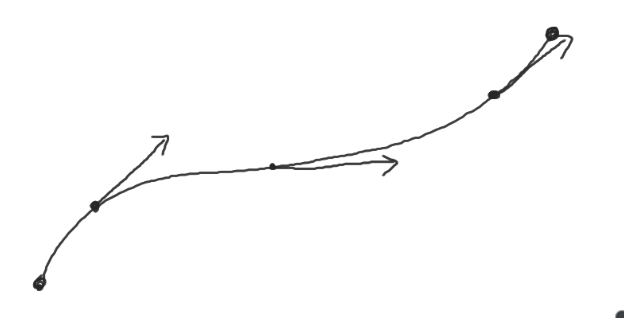
\includegraphics[width=0.35\textwidth]{images/00Fig12.png}};
      \end{tikzpicture}
      \caption{Streamline is just a flow of a vector field for at a fixed time $t$.}
      \label{fig:1.12}
    \end{figure}
    
    \begin{displaymath}
      M = \int_V \rho(\vec r, t) \d \vec r,
    \end{displaymath}
    \begin{displaymath}
      \ptf{M}{t} = \ptf{}{t} \in V \rho(\vec r, t) = \int_V \ptf{\rho(\vec r, t)}{t} \d \vec r.
    \end{displaymath}
    \begin{displaymath}
      \ptf{M}{t} = \int_V \ptf{\rho}{t} \d \vec r
      = -\int_{\partial V} \rho \vec u \cdot \vec n \d a,
    \end{displaymath}
    using Stokes theorem
    \begin{displaymath}
      = - \int_V \nabla \cdot (\rho \vec u)  \d \vec r.
    \end{displaymath}

    In other words
    \begin{displaymath}
      \int_V \left[ \ptf{\rho}{t} + \nabla \cdot (\rho \vec u) \right] \d \vec r = 0 ,
    \end{displaymath}
    and, since $V$ is arbitrary,
    \begin{displaymath}
      \ptf{\rho}{t} + \nabla \cdot (\rho \vec u) = 0.
    \end{displaymath}
    Which is called the \fnvi{continuity equation}.
    This is the general mass conservation, fluid can change density and so on.

\end{document}
